    \subsection*{What's still missing?}
    
        Last chapter, we used our linear regression model to do classification: we created a "hyperplane" to \textbf{separate} the the data that we placed in each class. 
    
        We also mentioned that regularization can increase \textbf{structural error}, by limiting what possible $\theta$ models we're allowed to use. 
            \note{Our goal was to decrease estimation error, but that's beside the point right now.}
    
        But, what if our linear model is already \textbf{too limited}? What if we need a more complicated model? This is true in a lot of real-world problems, like vibration:
    
        \begin{figure}[H]
            \centering
            
            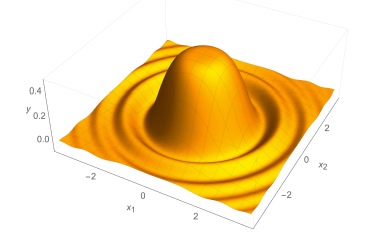
\includegraphics[width=70mm,scale=0.5]{images/feature_images/nonlinear_example.png}
            \caption*{This wave doesn't seem particular friendly to a planar approximation.}
        \end{figure}
    
        These kinds of situations are called, appropriately, \textbf{non-linear}.\\
    
        \begin{concept}
            \vocab{Non-linear} behavior cannot be accurately represented by any \gren{linear} model. 
    
            In order to create an accurate model, we have to use some \purp{nonlinear} operation.
        \end{concept}
    
        If we could create effective, non-linear models, we might even be able to deal with data that was previously "\textbf{linearly inseparable}".

    \subsecdiv

    \subsection*{Possible Solutions: Polynomials}

        Let's try to think of ways to approach this problem. We'll start with a 1-D input, for simplicity.

        Upon hearing "non-linear", we might remember the function we introduced last chapter: the \textbf{sigmoid}.
    
        \begin{figure}[H]
            \centering
            
            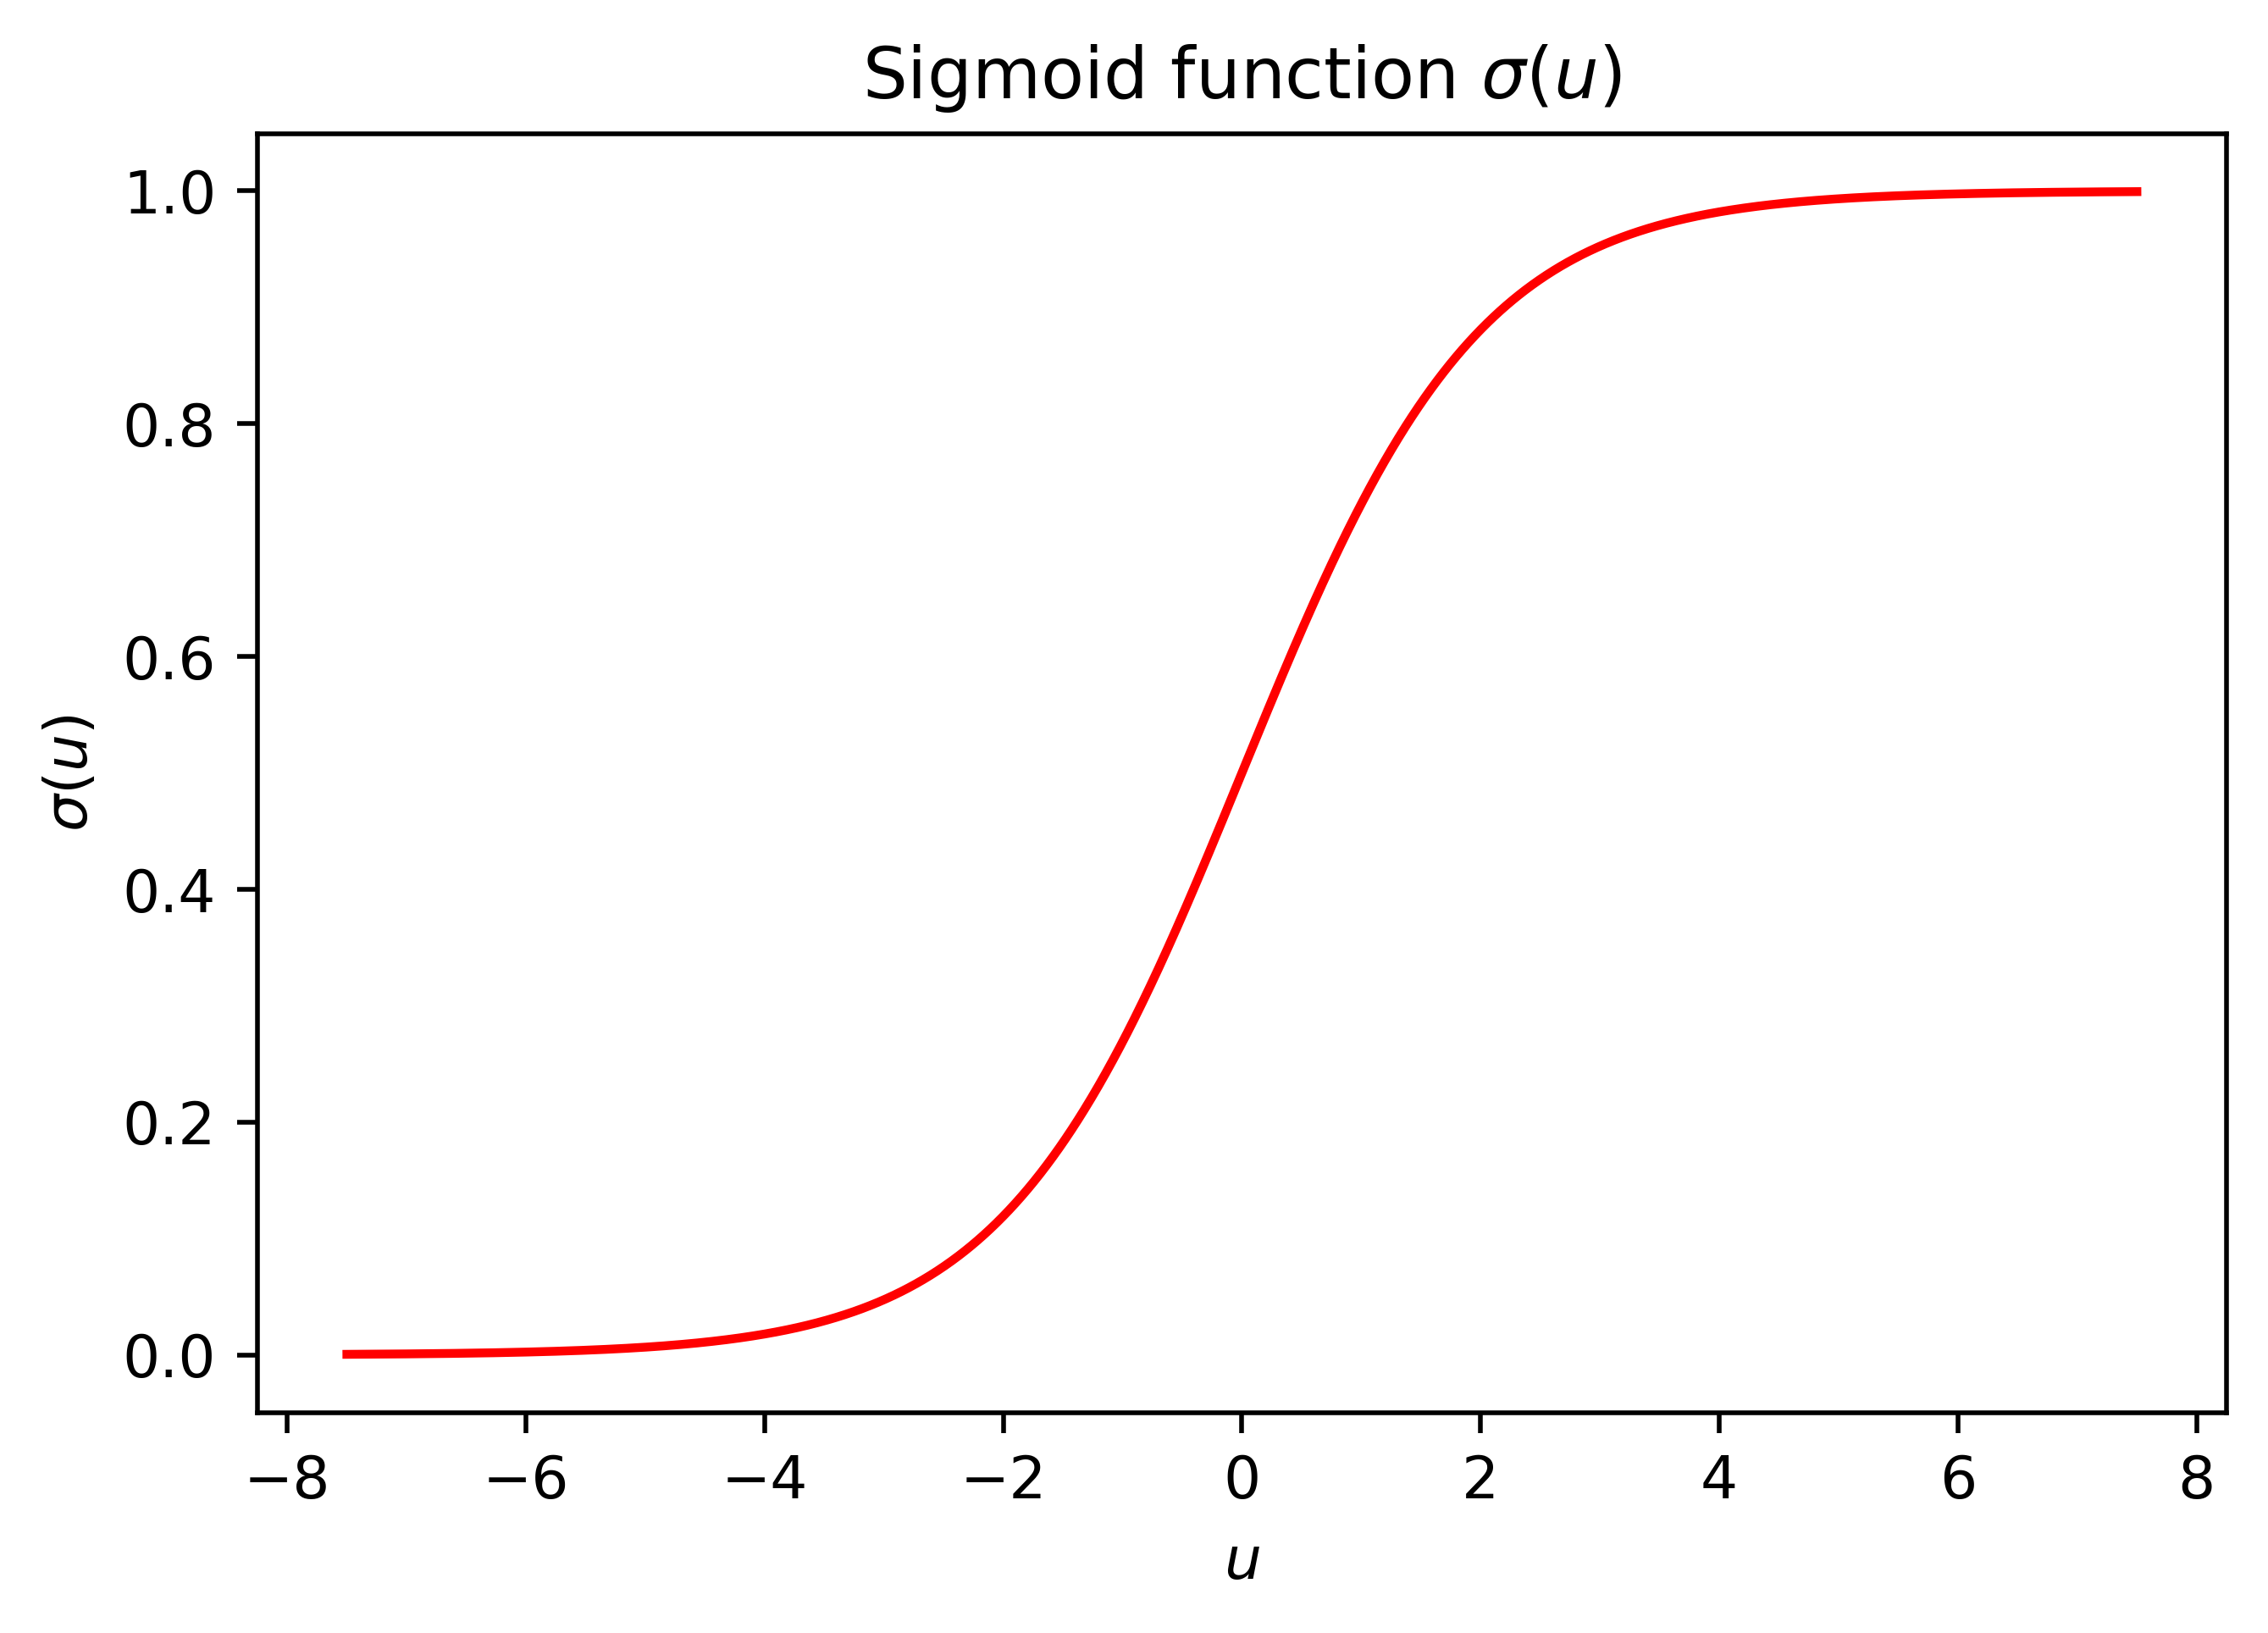
\includegraphics[width=70mm,scale=0.5]{images/feature_images/sigmoid_u.png}
            \caption*{Your friendly neighborhood sigmoid.}
        \end{figure}
    
        Can we use this to create a new model class? For now, unfortunately not: remember that we used this in the last chapter, and we still got a \textbf{linear} separator. The reasons were discussed there.
            \note{We'll show ways we can use this kind of approach, when we discuss Neural Networks.}
    
        Instead, we can get inspiration from our example of "structural error". For now, let's focus on \textbf{regression} (though classification isn't too different):
    
        \begin{figure}[H]
            
            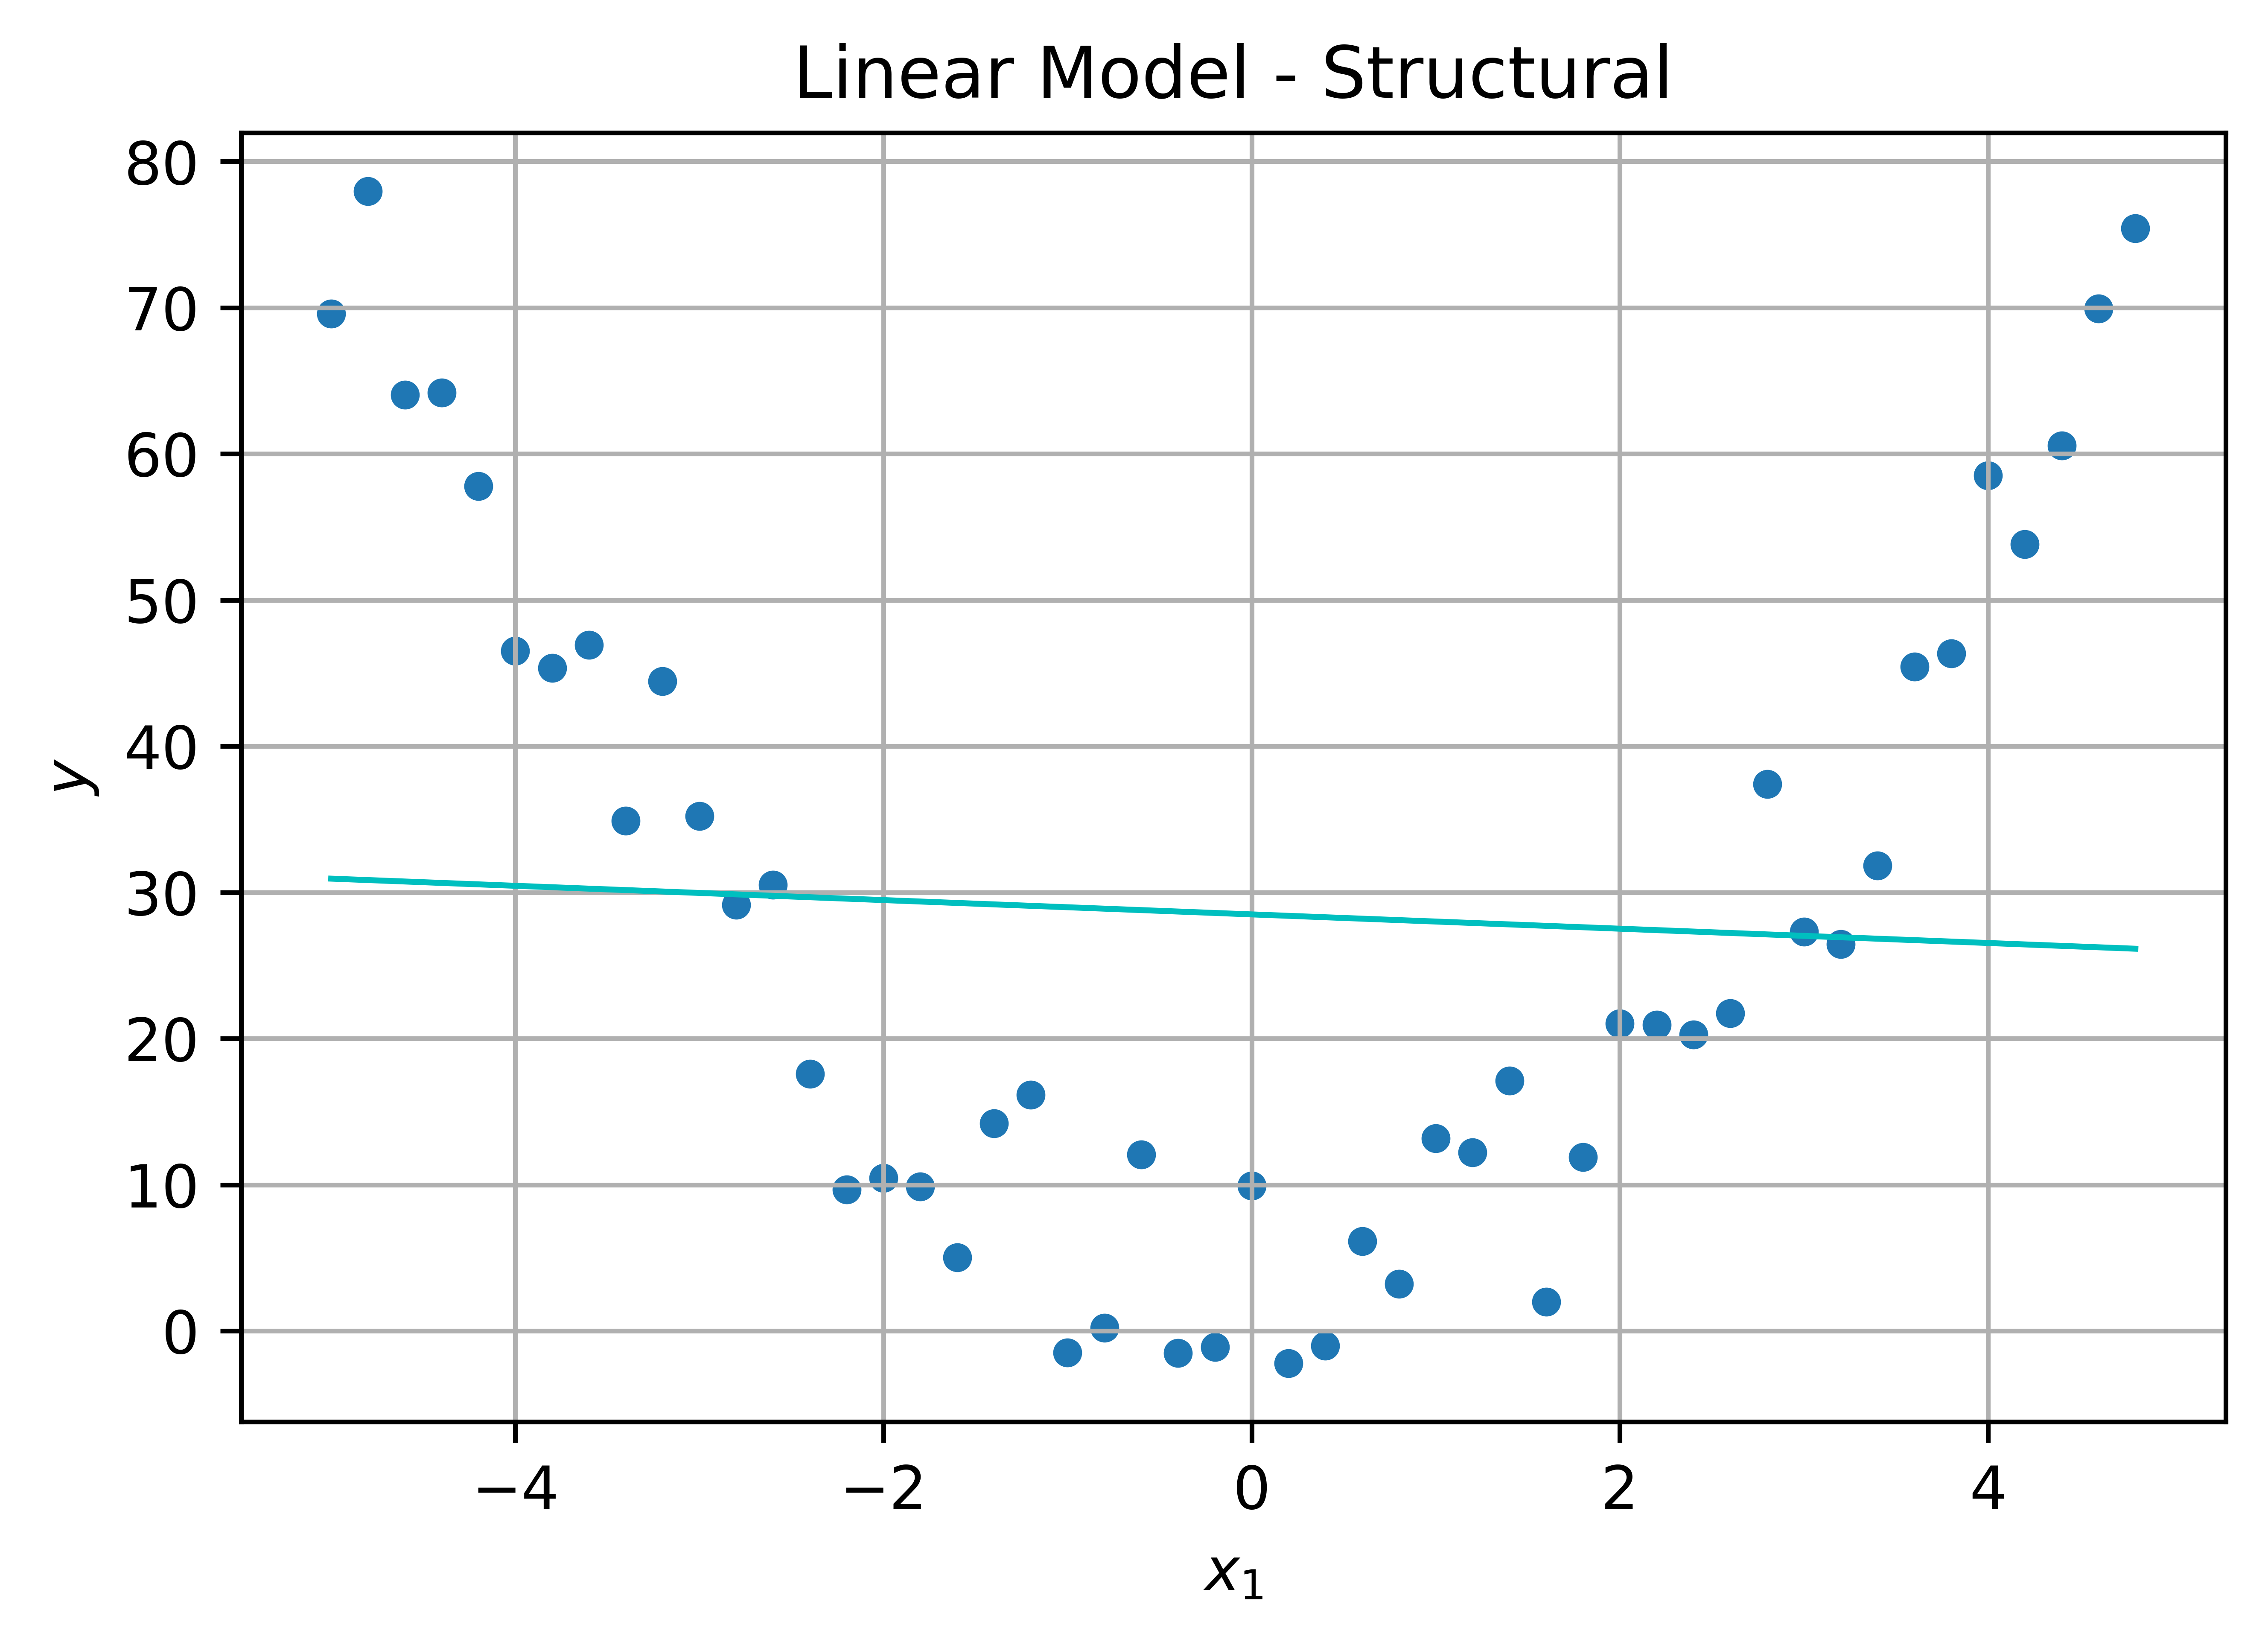
\includegraphics[width=70mm,scale=0.5]{images/feature_images/Structural_Linear_Model.png}
            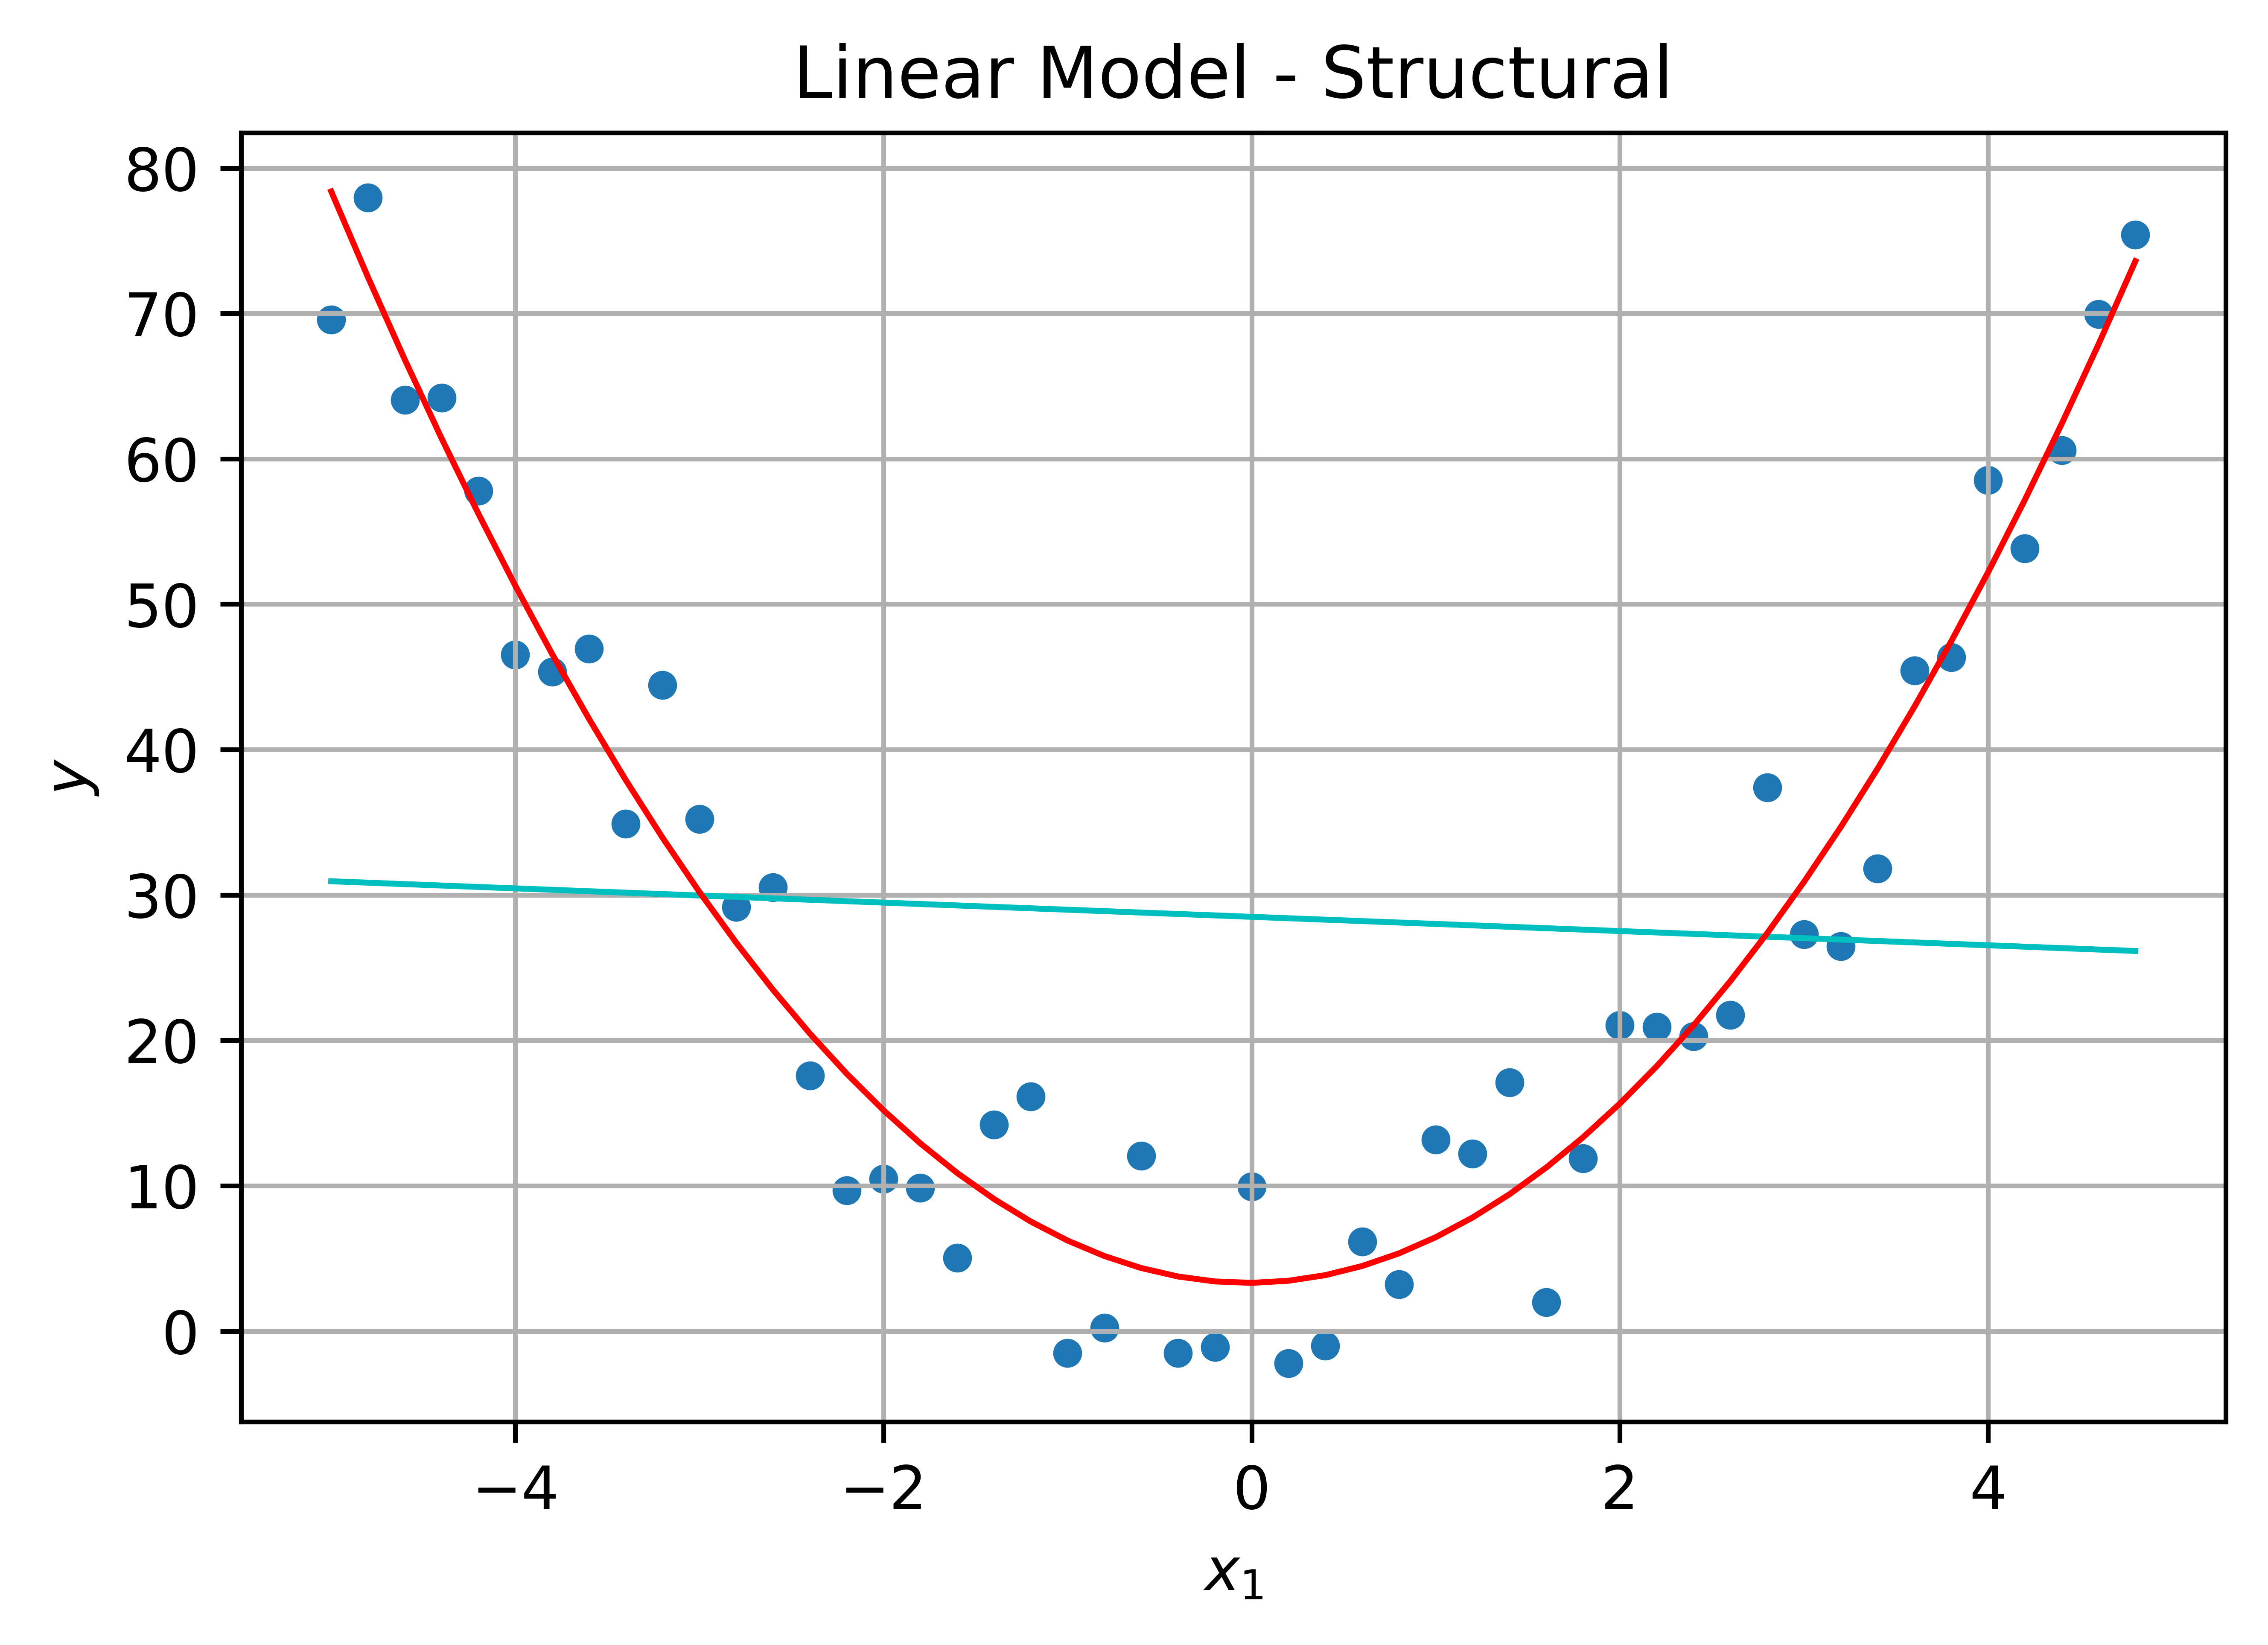
\includegraphics[width=70mm,scale=0.5]{images/feature_images/Structural_Quad_Model.png}
    
            \caption{A linear function can't represent this dataset. However, a parabola can!}
        \end{figure}
    
        We're still using our input variable $x$, but this time, we've "\textbf{transformed}" it: we have squared $x$, giving us a model of the form
            \note{Remember that $x$ is 1-D right now!}
    
        \begin{equation}
            h(x) = \red{A}x^2+\red{B}x+\red{C}
        \end{equation}
    
        It should be clear that his model is more \textbf{expressive} than the one before: it can create every model that our linear approach could (just by setting $A=0$), and it can create new models in a parabola shape.
            \note{Reminder: "expressiveness" or "richness" of a hypothesis class is how many models it can represent: a more expressive model can handle more different situations.}\\
    
        \begin{concept}
            We can make our \purp{linear} model more \gren{expressive} by add a squared term, and turning it into a \purp{parabolic} function.
    
            This concept can be extended even further, to any \vocab{polynomial}.
        \end{concept}

    \subsecdiv
    
    \subsection*{Transformation}
    
        How do we \textit{generalize} this concept? Well, we have a set of constant parameters $A, B, C$. These are similar to our constants $\theta_i$. Let's change our notation:
    
        \begin{equation}
            h(x) = \red{\theta_2} x^2 + \red{\theta_1} x + \red{\theta_0}
        \end{equation}
    
        Now, we've got something more familiar. We could imagine extending this to any number of terms $\theta_i x^i$: if we needed a cubic function, for example, we could include $\theta_3 x^3$.

        This is starting to look pretty similar to our previous model: in fact, we could even separate out $\theta$ as a variable:
            \note{Notice that $\theta_0$ corresponds to $x^0=1$.}

        \begin{equation}
            h(x) = 
            \overbrace{
                \sum_{i=1}^{k}
                \theta_i x^i
            }^{\text{Polynomial sum}}
            =
            \overbrace{
            \begin{bmatrix}
             \theta_0 \\ \theta_1 \\ \theta_2 \\ \vdots \\ \theta_k
            \end{bmatrix}
            \cdot 
            \begin{bmatrix}
                1 \\ x \\ x^2 \\ \vdots \\ x^k
            \end{bmatrix}
            }^{\text{Store as vectors}}
            = 
            \overbrace{
            \theta^T
            }^{\text{Simplify}}
            \begin{bmatrix}
                1 \\ x \\ x^2 \\ \vdots \\ x^k
            \end{bmatrix}
        \end{equation}

        This really \textit{is} starting to look like our linear transformation! That's helpful: we might be able to use the techniques we developed before.

        In fact, we can argue that they're \textbf{equivalent}: we've just changed what our input vector is. Consider our new input $\phi(x)$:

        \begin{equation}
            \blu{\phi(x)}
            = 
            \begin{bmatrix}
                1 \\ x \\ x^2 \\ \vdots \\ x^k
            \end{bmatrix}
            \qquad \qquad
            h(x) = 
            \red{\theta^T} 
            \overbrace{
            \blu{\phi(x)}
            }^{\text{New input}}
        \end{equation}
        
        This is called \textbf{transforming} our input.\\

        \begin{definition}
            A \vocab{transformation} $\phi(x)$ takes our input vector $x$ and converts it into a \gren{new} vector.

            This transformation can be used to:

            \begin{itemize}
                \item Allow our model to handle new, more \purp{complex} situations (more \gren{expressiveness})

                \item \purp{Pre-process} our data to make it \gren{easier} for our model to find \purp{patterns}.
                
                \item Convert our data into a \purp{usable} format (if, say, the original format doesn't fit into our equations)
                
            \end{itemize}
        \end{definition}

        \miniex Taking our input $x$ and converting it into a polynomial is a \textbf{transformation} of our input.

        This chapter will focus on these kinds of transformations. 

    \subsecdiv

    \subsection*{Features}
        
        One benefit of only changing out input is that we can continue to use our linear representation: we will be able to optimize a "linear" model $\theta$, over data that has been made \textbf{nonlinear}.

        These transformations can be complex, especially for multi-dimensional inputs. In this first case, we only combined one input with \textbf{itself}. But, often, we can combine multiple together!

        Thus, we should be careful to distinguish each input variable from each other. We often call these "\textbf{features}". However, we need to be careful:\\

        \begin{clarification}
            We often use the word \vocab{feature} in related (but not identical) contexts:

            \begin{itemize}
                \item A \vocab{feature} can be one \gren{aspect} of our \purp{original data}: for example, whether or not something is a cat or a dog, or the height of a patient. 

                \item A \vocab{feature} can also be one mathematical \gren{variable} in our \purp{transformed input}. $x_i$ is a feature of the data, while each variable of $\phi(x)$ is a feature of the transformed data.
            \end{itemize}

            Just like how we have an input space, we call the collection of possible values for our features the \vocab{feature space}.
        \end{clarification}

        \miniex $x$ in our previous example was a feature of the data, while $x^i$ is a feature of our transformed vector.
    
        Combined, this is why we called this technique the \textbf{feature transformation}: we apply some \textit{transform} to the \textit{features} of a data, to create a new set of \textit{features}.

        Since these transforms only apply to our features, we can keep the structure of a linear function:\\

        \begin{definition}
            \vocab{Feature transformation} allows us to do \gren{linear} regression or classification on a set of \purp{features} we have \gren{non-linearly} \purp{transformed}:

            \begin{equation*}
                h(x) = 
            \red{\theta^T} 
            \blu{\phi(x)}
            \end{equation*}

            $\phi(x)$ is our (often nonlinear) transformation of our features $x$.
        \end{definition}

    \secdiv